\documentclass[11pt]{article}
\usepackage{mathtools}
\usepackage{mdframed}
\usepackage{fullpage}
\usepackage{amsfonts}
\usepackage{tikz}
\usepackage{fancyhdr}
\usepackage{lastpage}
\usetikzlibrary{arrows,shapes,snakes,automata,backgrounds,petri, positioning}


%edit this for each class
\newcommand\name{John Collin Vincent}
\newcommand\classname{Com S 331}
\newcommand\assignment{Homework 9}


\newcounter{excounter}
\setcounter{excounter}{1}
\newcommand\ques[2]{\vskip 1em  \noindent\textbf{\arabic{excounter}\addtocounter{excounter}{1}.} \emph{#1} \noindent#2}
\newenvironment{question}{\ques{}\begin{quote}}{\end{quote}}


\pagestyle{fancy}
\rfoot{\name, page \thepage/\pageref{LastPage}}
\cfoot{}
\rhead{}
\lhead{}
\renewcommand{\headrulewidth}{0pt}
\renewcommand{\footrulewidth}{0pt}
\DeclarePairedDelimiter\ceil{\lceil}{\rceil}
\DeclarePairedDelimiter\floor{\lfloor}{\rfloor}


\begin{document}


  {\bf \classname \hspace{1cm} \assignment\hfill \name}
  \vskip 2em


  \begin{question}
    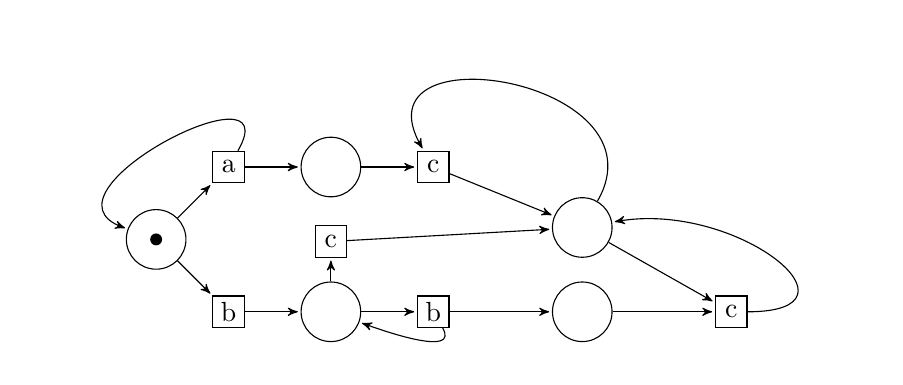
\begin{tikzpicture}[node distance=1.3cm,>=stealth',bend angle=45,auto]
      \node[place, tokens=1] (p1) {};
      \node[transition] (t1) [above right of = p1] {a};
      \node[transition] (t2) [below right of = p1] {b};
      \node[place] (p2) [right of=t1] {};
      \node[place] (p3) [right of = t2] {};
      \node[transition] (t3) [right of = p3] {b};
      \node[transition] (t4) [right of = p2] {c};
      \node[transition] (t5) [above = .3cm of p3] {c};
      \node[place] (p4) [right = of t3] {};
      \node[transition] (t6) [right = of p4] {c};
      \node[place] (p5) [above = .3 of p4] {};

      \path[->] (t1)
        edge [pre] (p1)
        edge [post] (p2)
        edge [post, out=60, in=160, looseness=2] (p1) ;
      \path[->] (t2)
        edge [pre]  (p1)
        edge [post] (p3);
      \path[->] (t3)
        edge [pre] (p3)
        edge [post] (p4)
        edge [post, out=300, in=-20] (p3);
      \path[->] (t4)
        edge [pre] (p2)
        edge [post] (p5)
        edge [pre, in=60, out=120, looseness=2] (p5);
      \path[->] (t5)
        edge [pre] (p3)
        edge [post] (p5);
      \path[->] (t6)
        edge [pre] (p4)
        edge [post, in=10, out=0, looseness=2] (p5)
        edge [pre] (p5);
    \end{tikzpicture}
  \end{question}


\end{document}
